% Layout for an independently distributed technical report.
\documentclass[manuscript,screen,nonacm]{acmart}
\setcopyright{none}
\settopmatter{printacmref=false,printccs=false}
\acmDOI{}
\acmISBN{}
\usepackage{longtable,booktabs,array,calc}
\usepackage{xurl}
\usepackage{fvextra}
\DefineVerbatimEnvironment{verbatim}{Verbatim}{breaklines=true,fontsize=\small}
\usepackage{tikz}
\usetikzlibrary{positioning}
\providecommand{\tightlist}{\setlength{\itemsep}{0pt}\setlength{\parskip}{0pt}}
\providecommand{\passthrough}[1]{#1}
\providecommand{\pandocbounded}[1]{#1}
\usepackage{graphicx,float}

% Permit figures to share pages with surrounding explanatory text.
\renewcommand{\topfraction}{0.92}
\renewcommand{\bottomfraction}{0.85}
\renewcommand{\textfraction}{0.06}
\renewcommand{\floatpagefraction}{0.80}
\setcounter{topnumber}{3}
\setcounter{bottomnumber}{3}
\setcounter{totalnumber}{5}
\setlength{\textfloatsep}{12pt plus 2pt minus 3pt}
\setlength{\intextsep}{12pt plus 2pt minus 3pt}
\raggedbottom

\geometry{top=0.75in,bottom=0.65in,includeheadfoot}
\begin{document}
\title{AFFECTOR-ARC: Emotional Trajectory Control through Transformer
Activation Steering}
\author{William Taggart}
\affiliation{\department{Modern and Classical Languages and Literatures}
\institution{Virginia Tech}\city{Blacksburg}\state{Virginia}\country{USA}}
\email{wtaggart@vt.edu}
\subtitle{Technical Report: November 13, 2026}
\begin{abstract}
AFFECTOR-ARC is an experimental command-line system for rewriting text
under a user-defined emotional trajectory. It runs a frozen Qwen3.5-0.8B
model on an NVIDIA GPU and changes selected internal activations during
generation. A trajectory specifies valence, inward/outward emotional
orientation, and intensity across normalized document position. Small
sets of contrasting English passages establish three activation
directions at each selected transformer layer. At inference time, the
requested coordinates determine a weighted displacement, scaled relative
to the current hidden-state magnitude, smoothed across decoding steps,
and constrained by an RMS budget. Paired hooks apply this displacement
to both the feed-forward input and its residual path. Document rewriting
combines these interventions with four editing styles, sentence-aware
segmentation, bounded generation, and incremental reporting. This report
derives the mechanism from its implemented operations and distinguishes
numerical controls from emotional outcomes. CPU policy tests pass; the
current revision still requires CUDA validation. No measured claim of
emotional accuracy, semantic preservation, or multilingual effectiveness
is made.
\end{abstract}
\keywords{activation steering, emotional text generation, transformer models, controllable generation}
\maketitle
\section{Literature review: activation steering and
emotion}\label{literature-review-activation-steering-and-emotion}

This focused review covers twelve papers, emphasizing 2025-2026 research
and retaining two methodological foundations. Titles, author lists,
version histories, and the claims summarized here were checked against
arXiv records and the corresponding paper text on November 13, 2026. The
cited versions are fixed below; availability on arXiv alone does not
establish peer review. The implications for this project are research
motivations, not evidence that its implementation reproduces these
results.

\textbf{From activation differences to behavioral control.} Activation
steering changes internal model states during inference while leaving
the backbone weights fixed. Turner et al.~derive intervention vectors
from contrasting prompts; Panickssery et al.~average differences across
positive and negative behavioral examples. These provide the
methodological basis for contrastive calibration, but do not validate a
particular emotional coordinate system or insertion site.
\citep{turner2023actadd}; \citep{panickssery2024caa}.

\textbf{Emotional expression and human judgment.} Wu et al.~relate model
emotion spaces to human valence/arousal judgments and report
concept-based steering across linguistic-cultural settings. Diallo et
al.~evaluate perceived emotional intensity and text quality with human
raters, finding that effects depend on emotion and steering strength.
Together they motivate separate measures of emotional movement and
readability. Their axes and numerical strengths cannot be assumed
equivalent to this project's inward/outward direction or RMS-scaled
controls. \citep{wu2025emotion}; \citep{diallo2026style}.

\textbf{Emotion can affect more than tone.} Sun et al.'s E-STEER uses
valence-arousal-dominance interventions to study reasoning, generation,
safety, and agent behavior, reporting non-monotonic relationships.
Jeong's small-model comparison reports both coherent emotional changes
and degeneration, including repetition, depending on extraction method
and architecture. These findings motivate reporting failed generations
alongside successes and testing strength sweeps rather than assuming
that larger perturbations improve emotional fit. Neither study
establishes an operating range for this implementation.
\citep{sun2026emotion}; \citep{jeong2026emotion}.

\textbf{Reading an emotion is different from controlling it.} Shu et
al.'s revised study identifies uneven causal organization of sparse
features across emotion categories and tests interventions for emotion
recognition. Wang et al.~show, in omni-modal models, that layers with
strong emotion-probing accuracy need not be the best intervention
layers. Recognition results therefore inform evaluator design, while
layer selection for rewriting still requires causal tests on generated
text. Neither finding licenses importing layer indices across
architectures. \citep{shu2026emotion}; \citep{wang2026readbest}.

\textbf{Multiple axes and adaptive control.} Ha et al.~find that
supportive-empathy directions are only partially separable: intervening
on one can shift other EPITOME proxy scores. Cui and Chen automate
vector extraction from labeled data, with task-dependent benefits.
Ferrando et al.~adapt intervention strength to context, studying the
balance between toxicity mitigation and retained utility. These
approaches motivate broader calibration, cross-axis tests, and future
adaptive control. The present coordinate mixture is not an
implementation of their learned selectors or context-dependent gates.
\citep{ha2026empathy}; \citep{cui2025pas}; \citep{ferrando2025dsas}.

\textbf{Evaluation must include costs as well as target effects.} Yang
et al.'s SteerScope evaluates steering efficacy jointly with side
effects, generalization, and data dependence. In its tested settings,
activation methods do not dominate prompt steering on the
efficacy/side-effect trade-off. For this project, the resulting
evaluation priorities are prompt-only and unsteered baselines, blinded
emotional and quality ratings, content-change assessment appropriate to
the rewrite style, and complete accounting of repetition, truncation,
and original-text fallbacks. This is an evaluation agenda, not a
completed benchmark. \citep{yang2026steerscope}.


\section{Problem and operating
principle}\label{problem-and-operating-principle}


\begin{figure}[!htb]
\centering
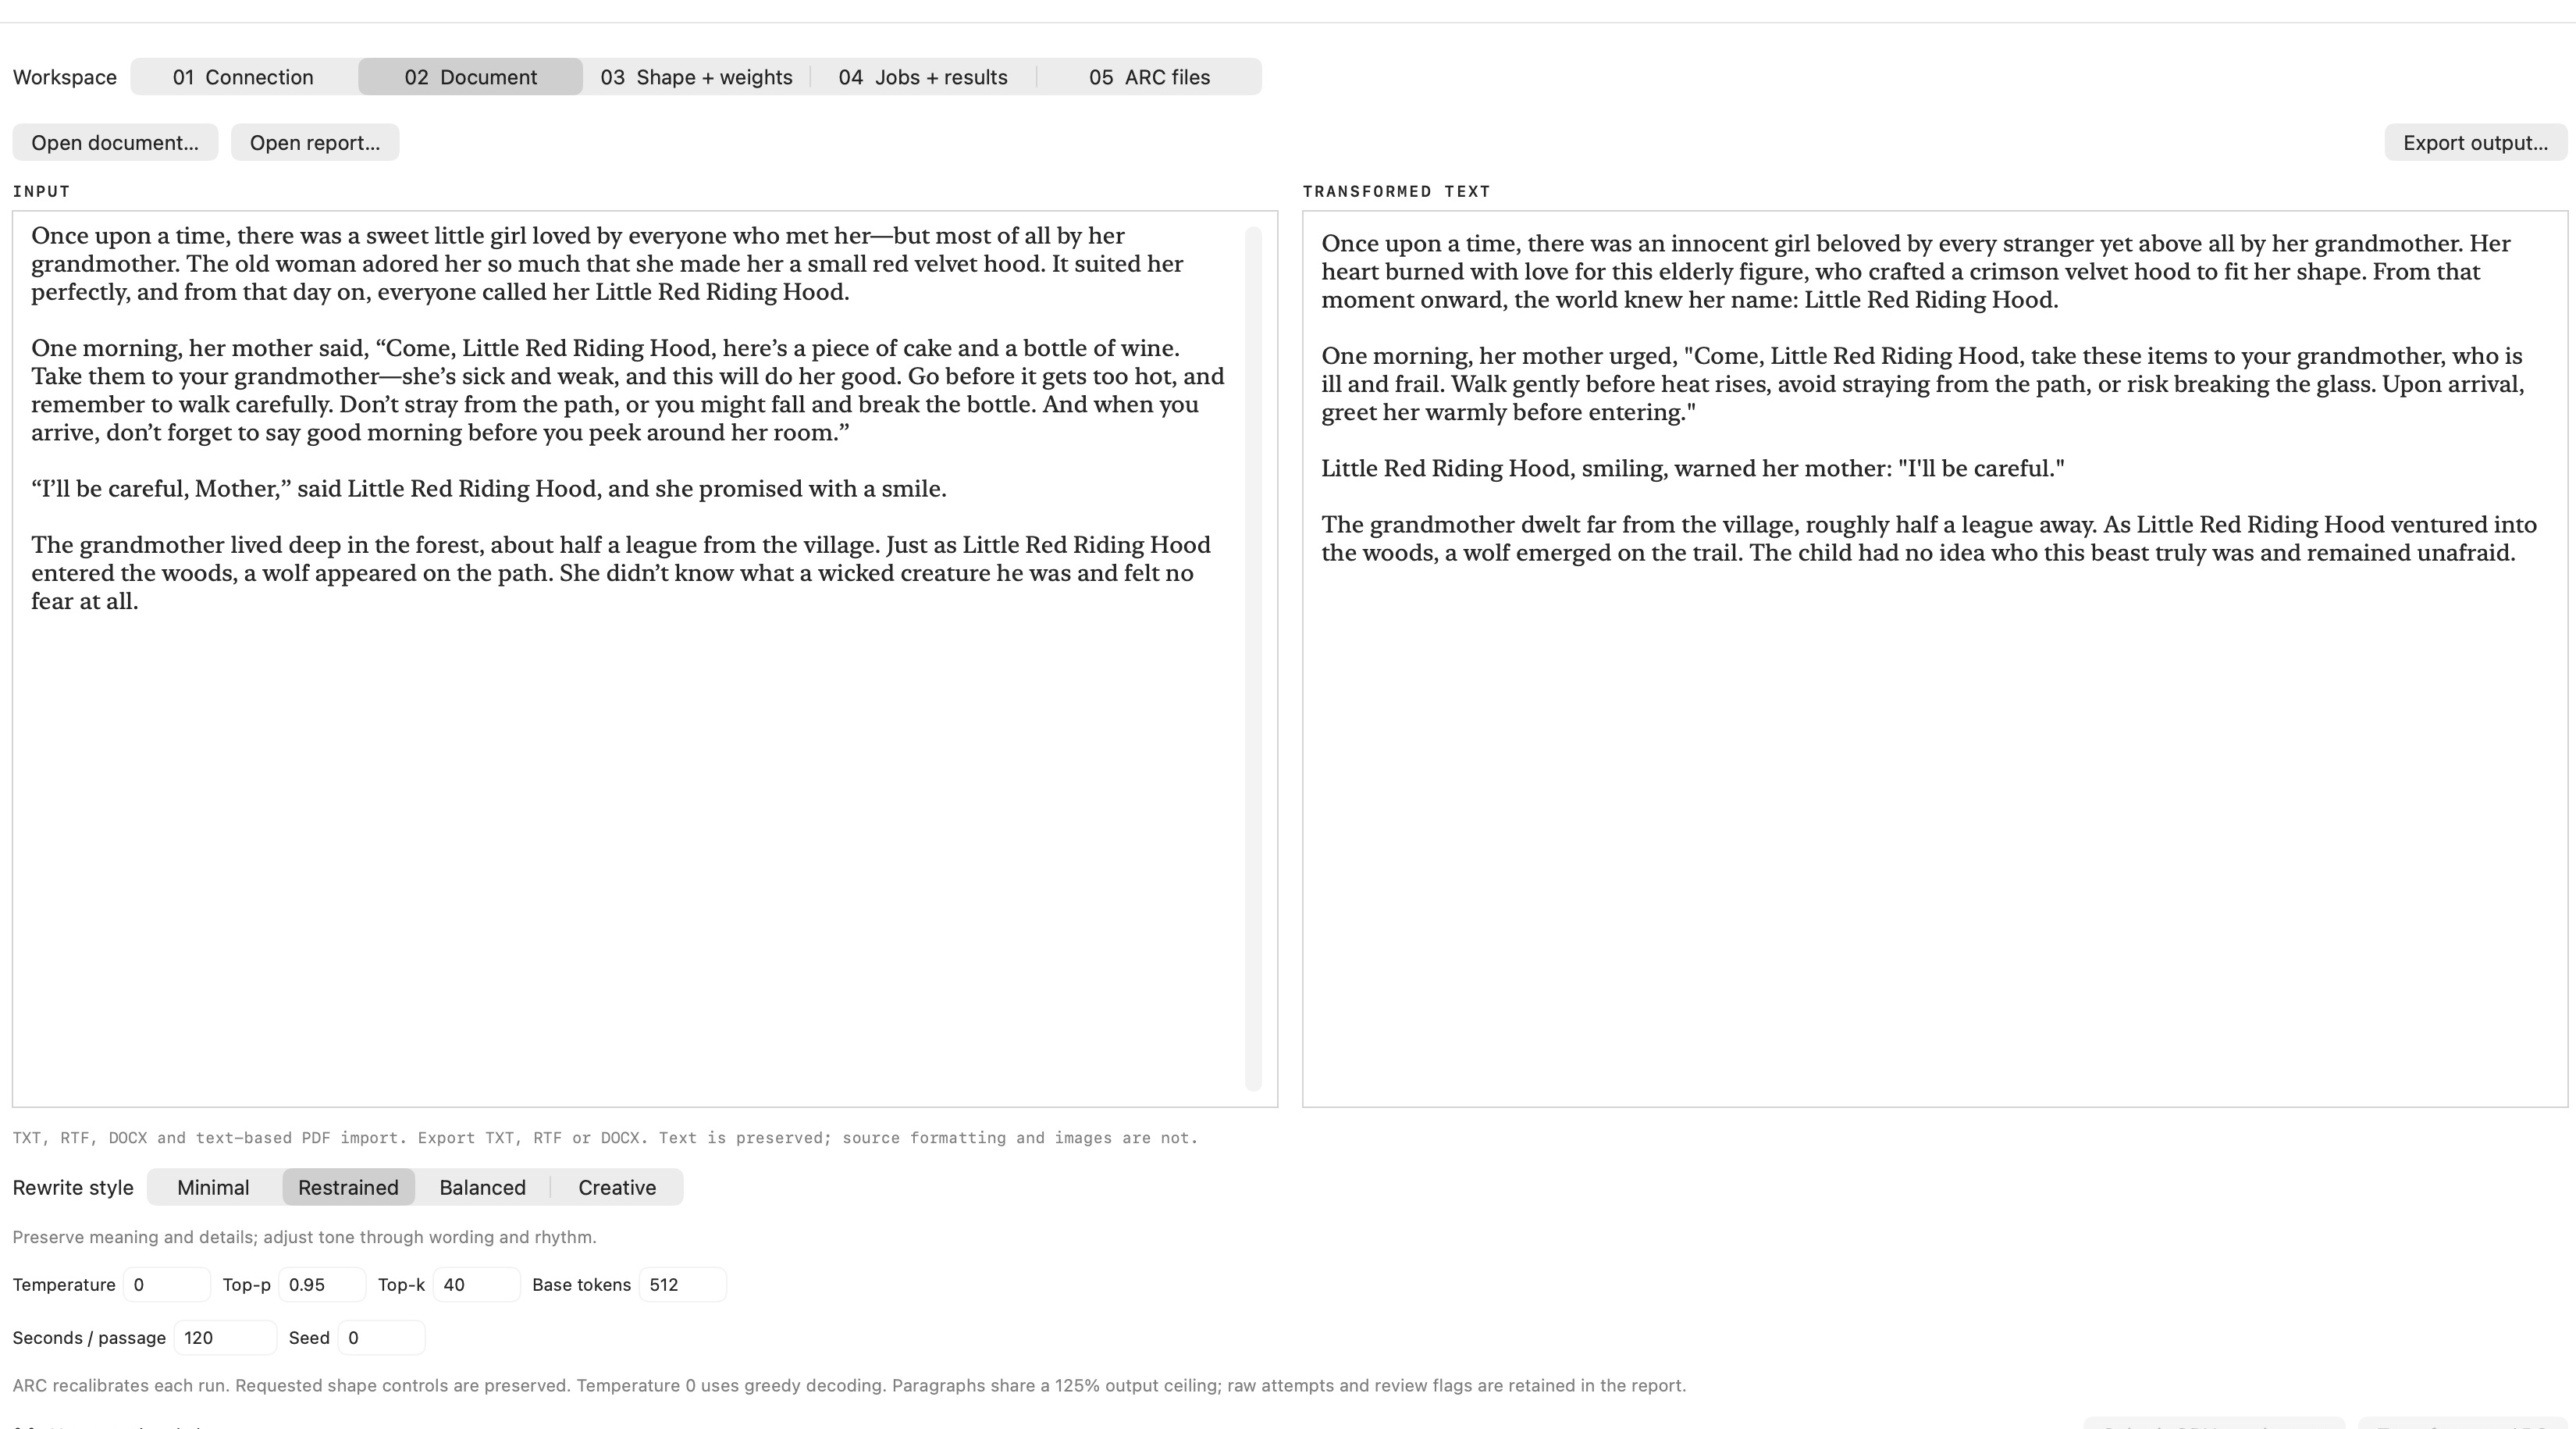
\includegraphics[width=\linewidth,height=0.58\textheight,keepaspectratio]{figures/screenshot-02.png}
\caption{Document workspace displaying an existing Little Red Riding Hood input and rewrite.}
\Description{Document workspace displaying an existing Little Red Riding Hood input and rewrite.}
\label{fig:app-screen-2}
\end{figure}
A language model generates text by repeatedly estimating a distribution
over the next token. Its intermediate hidden states are numerical
vectors that contribute to those estimates. Changing a hidden state can
change the continuation even when the input text and the model's stored
parameters remain fixed.

AFFECTOR-ARC uses this property to influence the emotional expression of
a rewrite. The user supplies an input document and a sequence of
emotional coordinates. The software maps positions in the input to
positions on that sequence, converts the coordinates into activation
displacements, and applies the displacements while generating each
rewritten passage.

The term \textbf{geometry} means an ordered path through a
three-dimensional coordinate space, together with layer settings and
optional calibration matrices. It does not mean that the software
reconstructs a solid surface or applies geometric constraints directly
to words. A text's emotional interpretation, a numerical target, and a
model's hidden states are distinct objects. The calibration is an
experimental mapping between them.

Two execution modes are available:

\begin{itemize}
\tightlist
\item
  \textbf{Rewrite:} process an entire UTF-8 text document in chunks,
  write the transformed text, and record attempts and failures.
\item
  \textbf{Smoke:} run five controlled generation conditions to check
  basic intervention and cleanup behavior.
\end{itemize}

The interface is a command-line runner for a CUDA allocation. It does
not provide a desktop interface, a hosted API service, automatic
emotional scoring, or conversational history.

\section{Runtime and data flow}\label{runtime-and-data-flow}


\begin{figure}[!htb]
\centering
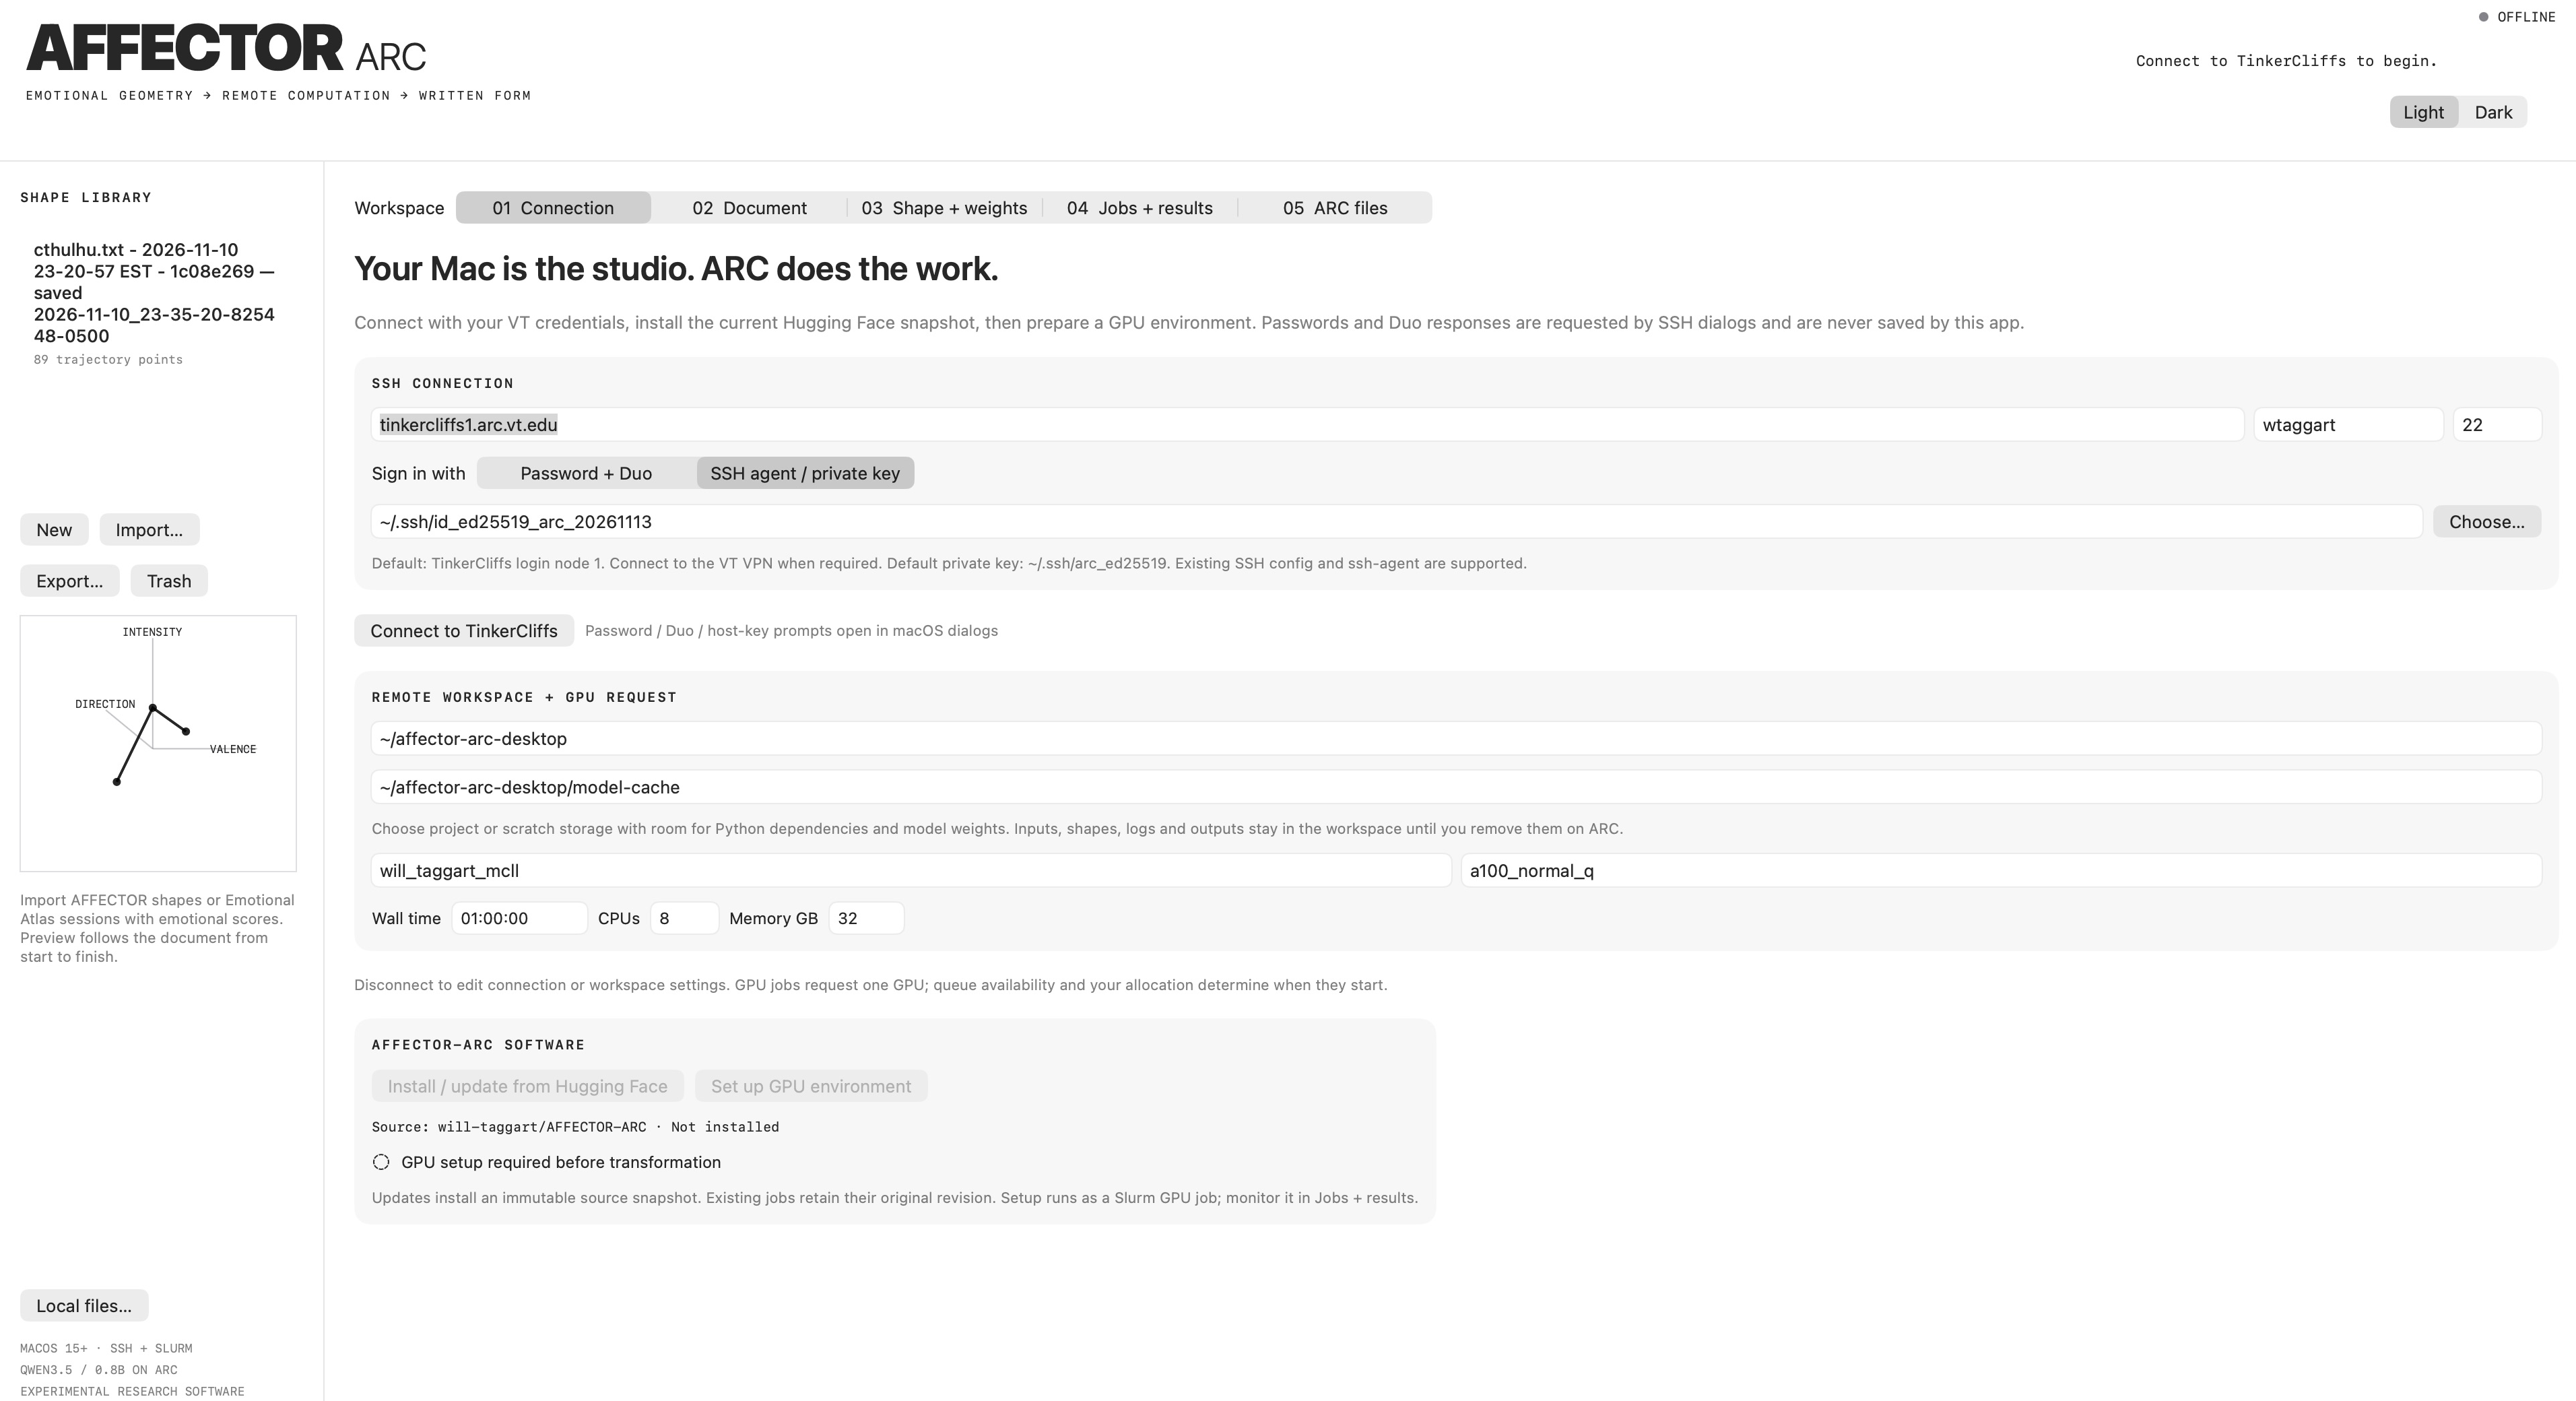
\includegraphics[width=\linewidth,height=0.58\textheight,keepaspectratio]{figures/screenshot-01.png}
\caption{Connection workspace with SSH settings and the Slurm GPU resource request. The client is offline in this capture.}
\Description{Connection workspace with SSH settings and the Slurm GPU resource request. The client is offline in this capture.}
\label{fig:app-screen-1}
\end{figure}
The runner loads \nolinkurl{Qwen/Qwen3.5-0.8B} at revision
\nolinkurl{2fc06364715b967f1860aea9cf38778875588b17}. The implementation
uses \nolinkurl{Qwen3_5ForConditionalGeneration}, its text decoder layers,
float32 computation, eager attention, and the first process-visible CUDA
device. It checks for 24 decoder layers; the geometry and calibration
code assume hidden width 1,024. The backbone is in evaluation mode, its
parameters have gradients disabled, and calibration and generation run
without gradient tracking.

The execution sequence is:

\begin{verbatim}
Read text and geometry settings
    → validate controls
    → load the pinned model on CUDA
    → calibrate the selected layers
    → select rewrite or smoke mode
    → generate with temporary activation hooks
    → remove hooks and save results
\end{verbatim}

Source files are distributed with the repository.
\nolinkurl{ENGINE_MANIFEST.json} records hashes for the bundled engine
snapshot. Model weights are downloaded separately. The setup script
creates a Python 3.12 environment, installs PyTorch from the CUDA 12.6
wheel index, pins Transformers to 5.22.2, runs the CPU policy tests, and
records installed packages in \nolinkurl{environment-resolved.txt}. PyTorch
and several support packages are resolved during setup rather than fully
locked in advance.

The example Slurm script requests one GPU, eight CPU cores, 64 GB of
host memory, and one hour. These are scheduling requests, not measured
minimum requirements. Users must supply an allocation and a suitable
model cache. The runner is single-process and single-GPU; it is not a
concurrent inference server.

\begin{figure}[!htb]
\centering
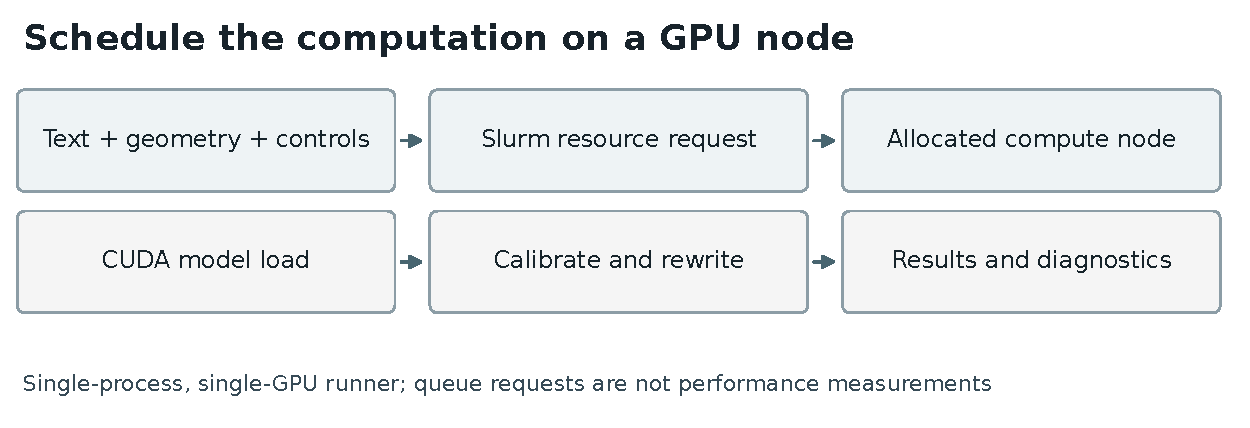
\includegraphics[width=\textwidth]{figures/illustration-01.pdf}
\caption{Execution schematic. The compute workload belongs to the allocated GPU node. Resource requests describe scheduling needs and do not establish measured minimum requirements.}
\Description{Schedule the computation on a GPU node. Execution schematic. The compute workload belongs to the allocated GPU node. Resource requests describe scheduling needs and do not establish measured minimum requirements.}
\label{fig:illustration-1}
\end{figure}

\section{Emotional coordinates and trajectory
interpolation}\label{emotional-coordinates-and-trajectory-interpolation}

A trajectory point is

\[
p_j=(t_j,v_j,d_j,i_j),
\]

where positions \(t_j\) increase strictly within \([0,1]\). Valence
\(v_j\) ranges from negative to positive in \([-1,1]\). Direction
\(d_j\) ranges from inward-oriented to outward-oriented emotion in
\([-1,1]\). Intensity \(i_j\) ranges from low to high in \([0,1]\).
Direction is an operational contrast concerning emotional orientation;
it is not dominance, speaker identification, or positive versus negative
sentiment.

Between adjacent points, the software linearly interpolates each
emotional coordinate. Before the first point and after the last, it uses
the endpoint values. The coefficient vector passed to the activation
module is

\[
c(t)=\bigl(v(t),d(t),2i(t)-1\bigr).
\]

Consequently, intensity 0.5 contributes a zero intensity coefficient;
intensity zero contributes a negative coefficient. These are control
conventions, not empirically established psychological units.

For a chunk occupying character offsets \([a,b)\) in an input of length
\(N\), its target is evaluated at

\[
t=\frac{a+b}{2N}.
\]

That target remains constant throughout generation of the chunk. A long
trajectory can therefore guide a short document without pairing source
and target paragraphs one to one. Only the positions sampled by the
target chunks are used; narrow changes between those positions may be
missed. The mapping uses original input positions, not positions in the
expanding or contracting output. Adjacent chunks receive separate
generation calls without prior rewritten chunks as conversational
context.

The runner accepts a native geometry JSON file and supported analysis
JSON structures containing emotional coordinates. It recalibrates the
basis on the current CUDA runtime even when the imported geometry
includes one. With no geometry argument, it uses a demonstration path
with three points; this path is not inferred from the input document.


\section{Estimating activation
directions}\label{estimating-activation-directions}

A hidden state at a selected layer is a vector in \(\mathbb{R}^{1024}\).
To estimate a direction associated with one emotional contrast, the
system compares the model's states for paired passages that differ in
the desired property.

There are four hand-authored English pairs for each of three axes. For
layer \(\ell\), axis \(j\), and pair \(k\), let \(h^+_{\ell,j,k}\) and
\(h^-_{\ell,j,k}\) denote the captured states for the two members. The
mean difference is

\[
u_{\ell,j}=\frac14\sum_{k=1}^{4}
\left(h^+_{\ell,j,k}-h^-_{\ell,j,k}\right).
\]

For a vector of dimension \(D\), define root-mean-square magnitude as

\[
\operatorname{RMS}(x)=\sqrt{\frac1D\sum_{r=1}^{D}x_r^2}.
\]

The normalized direction is

\[
b_{\ell,j}=\frac{u_{\ell,j}}
{\max(\operatorname{RMS}(u_{\ell,j}),10^{-8})}.
\]

The three directions form the rows of a matrix
\(B_\ell\in\mathbb{R}^{3\times1024}\). Calibration captures the final
chat-formatted prompt position immediately before
\nolinkurl{post_attention_layernorm}. It does not average all token
positions. All selected layers are captured during the same 24 forward
passes: three axes, four pairs, and two members per pair.

Default layers are 8, 16, and 23, using zero-based indexing, with
weights 1, 1, and 0.5. This is subtraction, averaging, and
normalization; there is no training optimizer, backbone fine-tuning,
orthogonalization, or outcome-based fitting. The small calibration set
may encode vocabulary, topic, or perspective along with emotion.
Normalizing the vectors does not establish that the axes are independent
or valid across languages.


\section{From coordinates to bounded
displacements}\label{from-coordinates-to-bounded-displacements}


\begin{figure}[!htb]
\centering
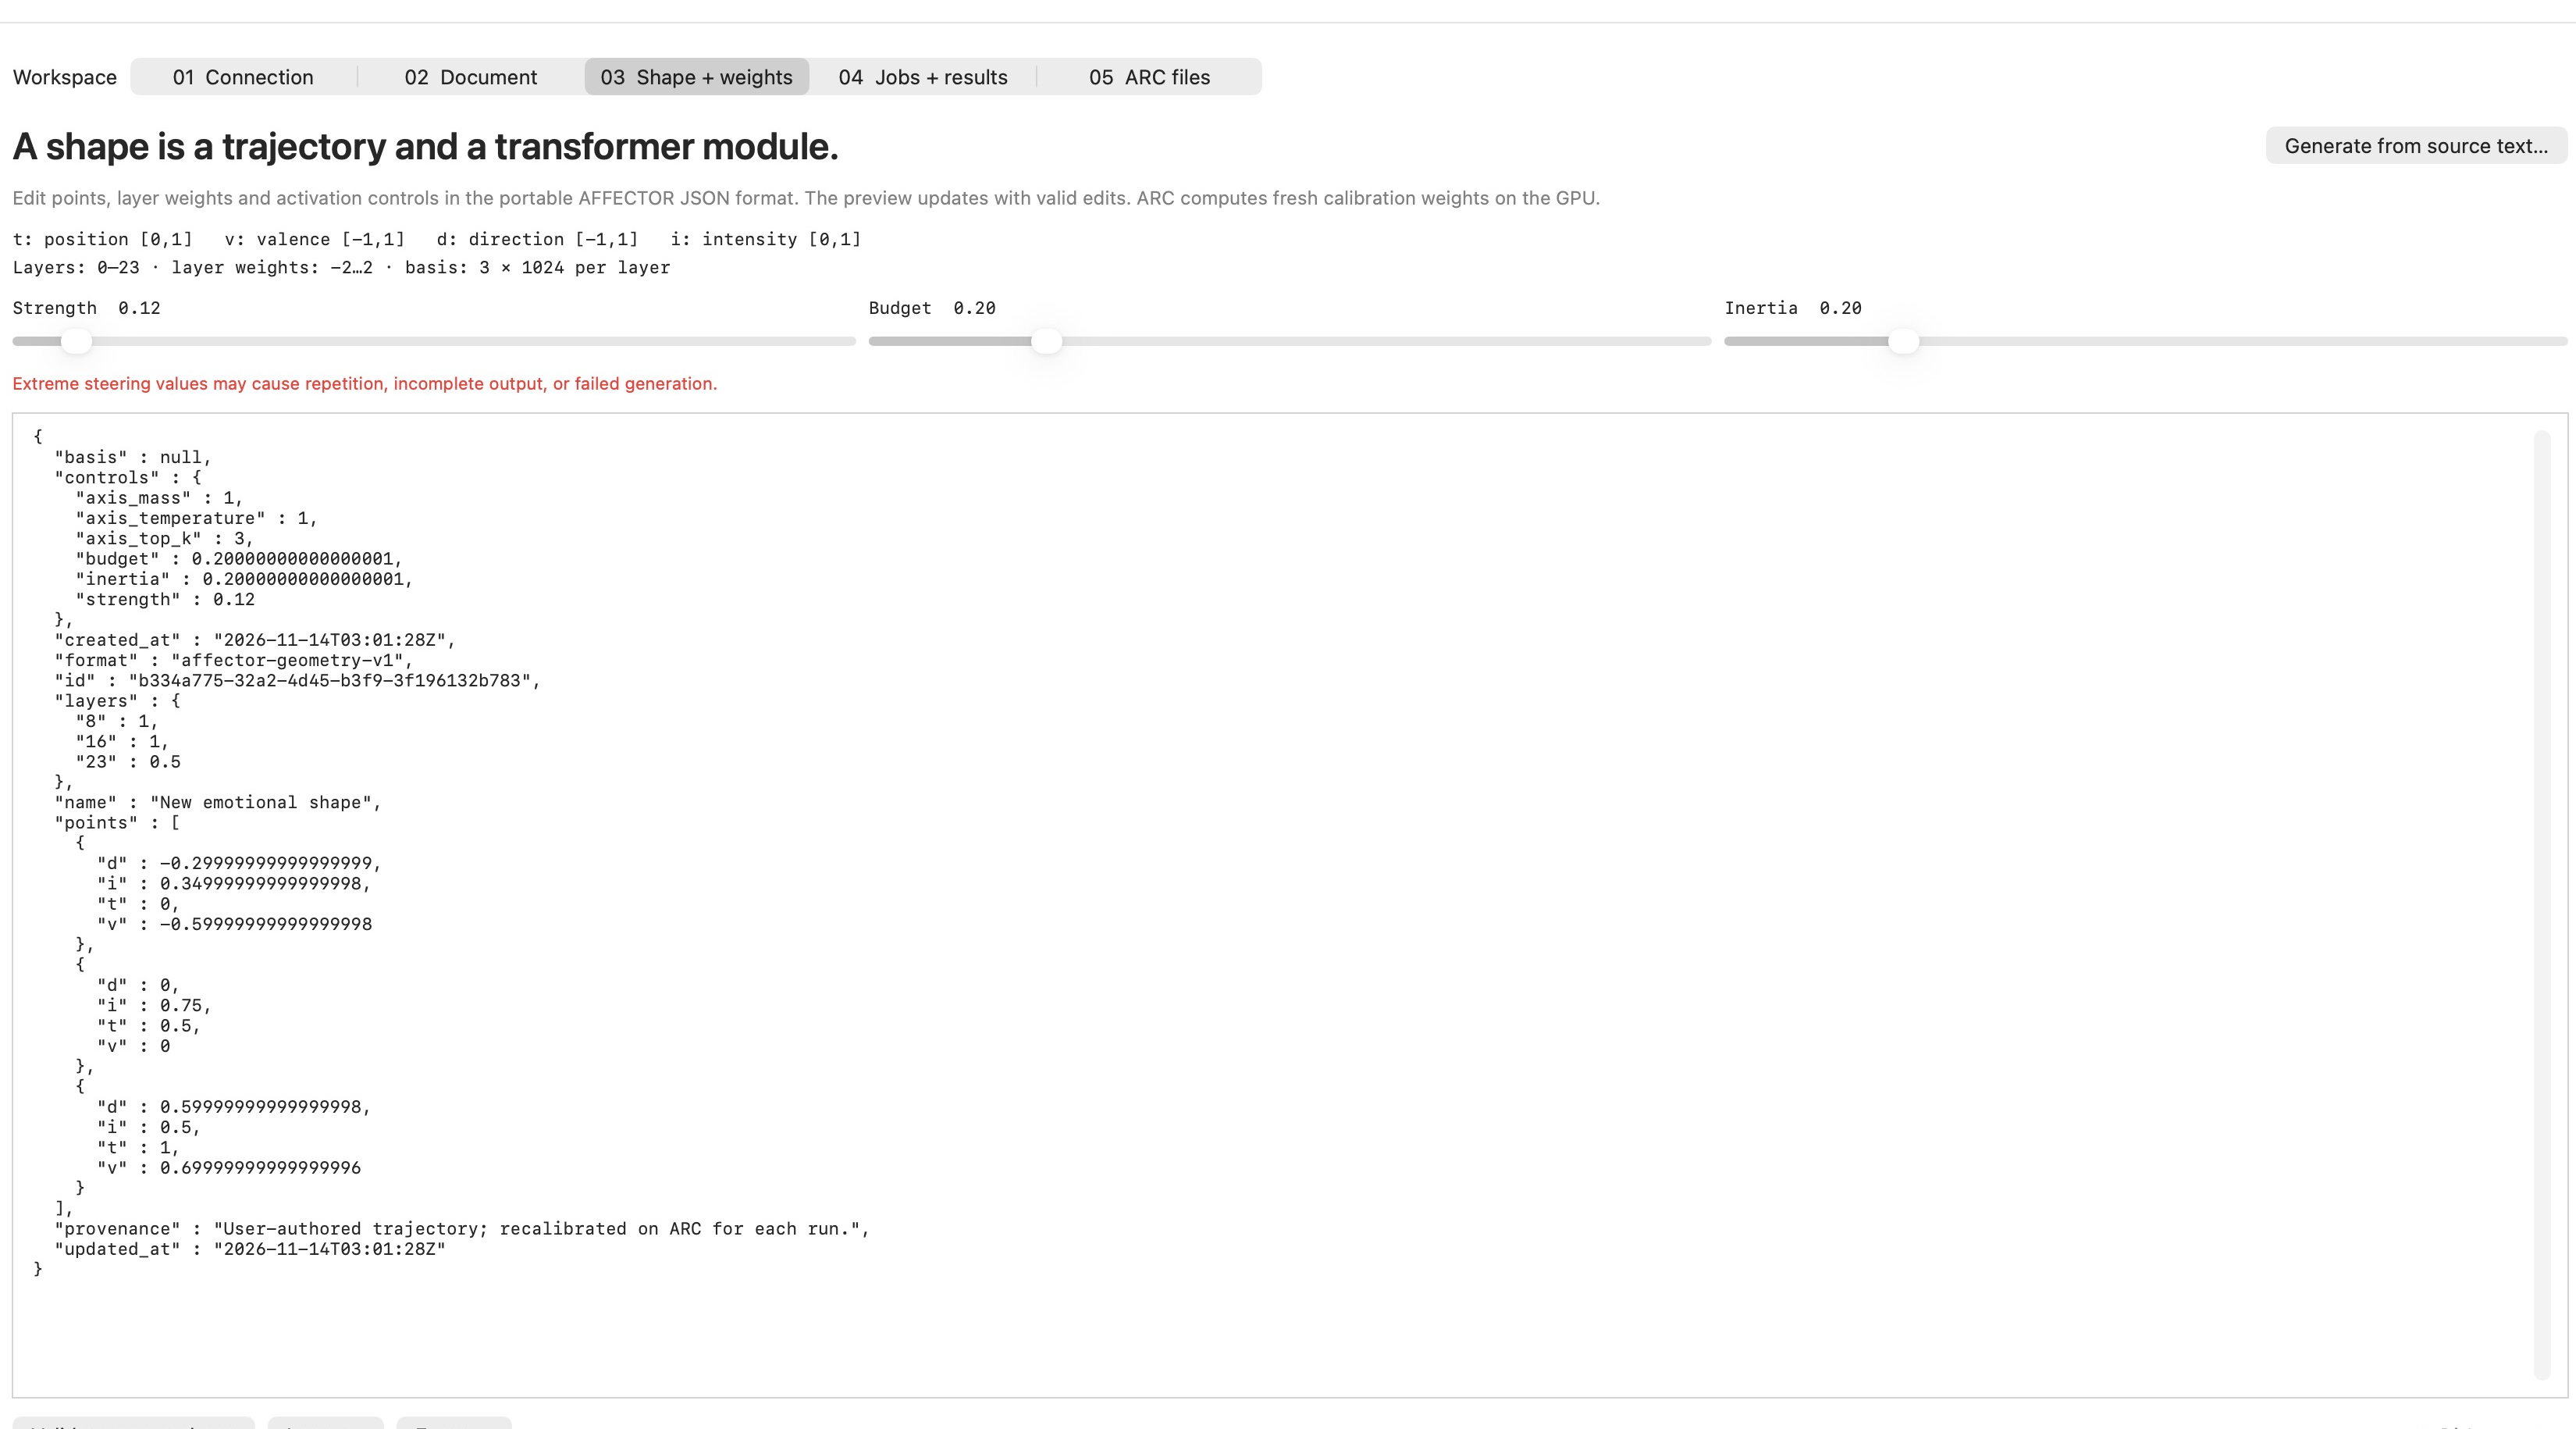
\includegraphics[width=\linewidth,height=0.58\textheight,keepaspectratio]{figures/screenshot-03.png}
\caption{Geometry and weights editor with the trajectory and activation-steering controls.}
\Description{Geometry and weights editor with the trajectory and activation-steering controls.}
\label{fig:app-screen-3}
\end{figure}
\subsection{Selecting and weighting
axes}\label{selecting-and-weighting-axes}

Let \(T\) be axis temperature. Each coordinate first receives magnitude

\[
q_j=|c_j|^{1/T}.
\]

Axes are sorted by this magnitude. The algorithm retains at most
\nolinkurl{axis_top_k} axes and stops adding axes after their accumulated
magnitude reaches \nolinkurl{axis_mass} times the total magnitude.
Selection includes the axis that crosses the threshold. The retained
coefficients are

\[
a_j=\operatorname{sign}(c_j)q_jm_j,
\]

where \(m_j\) is one for a retained axis and zero otherwise.
Coefficients are not renormalized after selection. For coordinate
magnitudes below one, \(T<1\) reduces their magnitudes and emphasizes
relative differences; \(T>1\) increases them and makes those differences
less pronounced. These operations affect three activation coefficients,
not token probabilities.

\subsection{Strength, inertia, and
budget}\label{strength-inertia-and-budget}

For the current final-token state \(h_{\ell,n}\), strength \(s\), and
layer weight \(w_\ell\), the raw displacement is

\[
r_{\ell,n}=s\,w_\ell\operatorname{RMS}(h_{\ell,n})(aB_\ell).
\]

Multiplication by the current state's RMS expresses the intervention
relative to the layer's numerical scale. A negative layer weight
reverses the mixed direction at that layer.

On the first decoding step, the smoothed displacement equals
\(r_{\ell,n}\). On later steps, inertia \(\rho\) combines the previous
applied displacement with the new raw displacement:

\[
\widetilde\delta_{\ell,n}=\rho\delta_{\ell,n-1}+(1-\rho)r_{\ell,n}.
\]

Budget \(\beta\) then limits the RMS ratio:

\[
\delta_{\ell,n}=\widetilde\delta_{\ell,n}
\min\left(1,
\frac{\beta\operatorname{RMS}(h_{\ell,n})}
{\max(\operatorname{RMS}(\widetilde\delta_{\ell,n}),10^{-12})}
\right).
\]

Strength determines the proposed displacement; budget supplies its
ceiling. Raising the budget has no effect when the proposed displacement
already fits below it. Budget 1 permits a displacement as large in RMS
as the hidden state itself. It is not a token allowance, a
semantic-change quota, or a guarantee of stronger emotional accuracy.
Inertia uses the previous already-capped displacement and resets with
each new generation call.

\subsection{Intervention site}\label{intervention-site}

Let \(h\) denote the state entering the feed-forward portion of a
decoder block. Without intervention, that portion computes

\[
y=h+\operatorname{FFN}(\operatorname{Norm}(h)).
\]

The implemented intervention produces

\[
y=(h+\delta)+\operatorname{FFN}(\operatorname{Norm}(h+\delta)).
\]

A pre-hook adds \(\delta\) to the normalization input; a block-output
hook adds the same displacement to the residual result. Adding a vector
only after an unchanged feed-forward computation would have a different
effect. Only the final prompt position is modified during prefill;
cached decoding modifies the current generated position. The module does
not wait for specific words or phrases. Generation hooks are removed in
a \nolinkurl{finally} block.

This is an open-loop intervention. Coefficients come from the requested
absolute coordinates, not the difference between a measured output
emotion and the target. A zero coefficient adds no intervention on that
axis; it does not actively neutralize emotion already expressed by the
model.


\section{User controls and rewrite
instructions}\label{user-controls-and-rewrite-instructions}

{ % do not increment counter
\begin{longtable}[]{@{}
  >{\raggedright\arraybackslash}p{(\linewidth - 4\tabcolsep) * \real{0.3000}}
  >{\raggedleft\arraybackslash}p{(\linewidth - 4\tabcolsep) * \real{0.4000}}
  >{\raggedright\arraybackslash}p{(\linewidth - 4\tabcolsep) * \real{0.3000}}@{}}
\toprule\noalign{}
\begin{minipage}[b]{\linewidth}\raggedright
Control
\end{minipage} & \begin{minipage}[b]{\linewidth}\raggedleft
Default without an imported override
\end{minipage} & \begin{minipage}[b]{\linewidth}\raggedright
Function
\end{minipage} \\
\midrule\noalign{}
\endhead
\bottomrule\noalign{}
\endlastfoot
Strength & 0.12 & Scale the proposed activation displacement \\
Budget & 0.20 & Cap displacement RMS relative to hidden-state RMS \\
Inertia & 0.20 & Weight the preceding applied displacement \\
Axis top-k & 3 & Maximum number of retained emotional axes \\
Axis mass & 1.0 & Cumulative magnitude threshold for axis selection \\
Axis temperature & 1.0 & Exponent control for emotional-axis
magnitudes \\
Temperature & 0 & Select greedy decoding or token sampling \\
Top-p & 0.95 & Probability-mass cutoff when sampling \\
Top-k & 40 & Token candidate count when sampling \\
Base output tokens & 512 & Initial generation allowance, expanded in
rewrite mode \\
Time limit & 120 seconds & Per-generation stopping threshold \\
\end{longtable}
}

The CLI overrides only the activation settings explicitly supplied;
other settings come from the imported geometry or defaults. Validation
permits strength 0--2, budget 0--1, inertia 0--0.99, axis top-k 1--3,
axis mass 0.01--1, and axis temperature 0.1--3. These accepted ranges
are not validated operating recommendations. The terminal displays the
warning: \textbf{Extreme values for strength, budget, and inertia may
cause generation failures.}

At temperature zero, decoding is greedy and top-p/top-k are inactive. At
positive temperature, they affect token selection after the model
computes its scores. They do not replace or modify the three-axis
activation selection mechanism.

Four system-prompt styles provide separate editing constraints:

\begin{itemize}
\tightlist
\item
  \textbf{Minimal:} change a few words or phrases while preserving
  nearly all wording and sentence order.
\item
  \textbf{Restrained:} adjust tone through wording, rhythm, and emphasis
  while preserving central meaning, facts, terminology, and structure;
  invent no scenes or metaphors.
\item
  \textbf{Balanced:} allow a clearer emotional shift and modest
  figurative language while retaining central meaning, facts, people,
  and events.
\item
  \textbf{Creative:} permit changes to meaning, imagery, and events,
  while requesting concise output in the same language.
\end{itemize}

Restrained is the default in rewrite mode. Smoke mode retains its
original general rewriting instruction unless a style is explicitly
selected. Each prompt requests complete sentences and treats supplied
text as material rather than instructions. A per-chunk suffix specifies
the original character count and hard character allowance. Numerical
emotional coordinates are not inserted into these prompts; the
coordinates act through hidden states. Prompt instructions influence
generation but are not formal semantic guarantees. The runner has no
semantic-equivalence rejection filter and does not lower steering
settings automatically.

\section{Segmentation, length control, and
repetition}\label{segmentation-length-control-and-repetition}

The runner reads and trims the outer whitespace of a UTF-8 text file.
Blank lines define paragraphs. Long paragraphs are split using a
700-character ceiling, preferring sentence punctuation when a suitable
boundary exists, then whitespace, and finally a hard split. This is a
punctuation heuristic, not a linguistic sentence parser. Original
whitespace between chunks is preserved during output assembly.

Within each original paragraph, the character ceiling is 125\% of the
original span processed so far. If \(s\) is the first chunk's start,
\(b_j\) the current chunk's end, and \(U_j\) the output characters and
intervening whitespace already used, the current allowance is

\[
L_j=\max\left(0,\left\lfloor1.25(b_j-s)\right\rfloor-U_j\right).
\]

Unused allowance carries forward within that paragraph. It cannot be
borrowed from future chunks or transferred across a blank-line paragraph
boundary. Character counts are Python string lengths, not word counts,
encoded byte counts, or model-token counts.

Generation aims for the original length. Starting at 85\% of the current
input chunk's characters, a recognized sentence ending can stop
generation. A separate hard character threshold prevents excessive
expansion. The token allowance is

\[
K_j=\min\left(2048,\max(K_{\mathrm{base}},L_j)\right),
\]

which supplies decoding headroom but does not imply one token equals one
character. The time threshold is checked between decoding steps and
cannot interrupt a blocked GPU kernel immediately.

Decoding also uses a repetition penalty of 1.1 and an eight-token
no-repeat n-gram constraint. A text-level detector checks every eight
generation steps for repeated three- to six-word sequences appearing at
least four times in the last 100 words, or a short compact character
pattern repeated at least six times in the last 240 characters. These
heuristics can miss some loops and can flag intentional repetition.

After a generation attempt, the runner checks for repetition, empty
output, excessive length, and an unfinished ending. A problematic draft
is reduced to a complete, nonrepetitive sentence prefix within its
allowance. If none exists, the original chunk is retained and flagged.
The returned draft remains in the report's attempt record before
sentence salvage. However, the engine has already clipped it to the hard
character allowance; the report is not a lossless record of characters
beyond that boundary.

Sentence cleanup prevents chopped words from being joined directly to
the next passage, but it may omit ideas from the tail of a draft.
Neither punctuation recognition nor output-size compliance establishes
completeness of meaning.

\section{Failure handling and output
artifacts}\label{failure-handling-and-output-artifacts}


\begin{figure}[!htb]
\centering
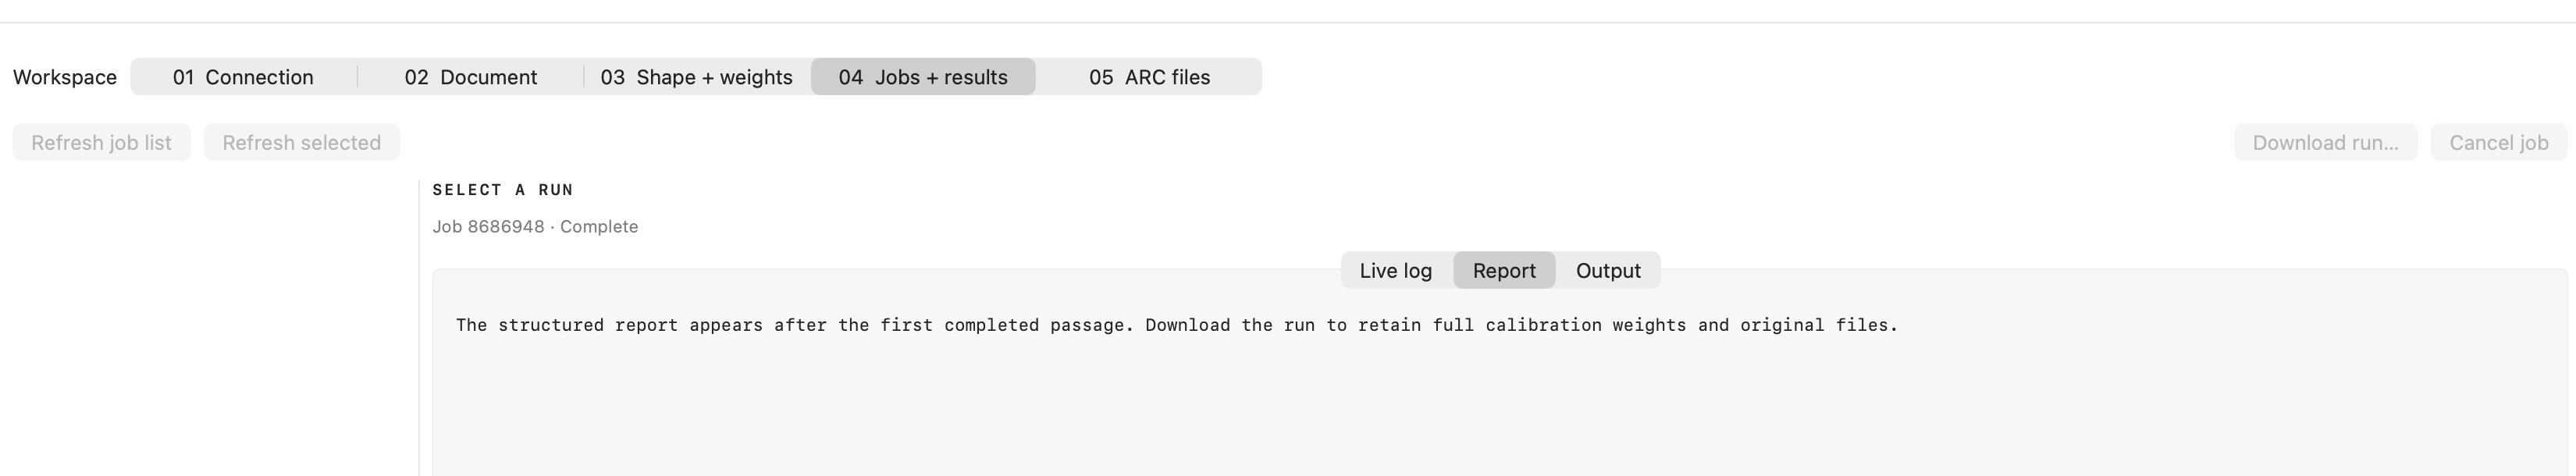
\includegraphics[width=\linewidth,height=0.58\textheight,keepaspectratio]{figures/screenshot-04.png}
\caption{Jobs and results controls in the offline client; the report pane has no loaded report.}
\Description{Jobs and results controls in the offline client; the report pane has no loaded report.}
\label{fig:app-screen-4}
\end{figure}
Each chunk receives one generation attempt at the requested activation
settings. A caught generation exception is recorded; the original chunk
remains in the assembled text and processing continues. Calibration
failures, invalid inputs, filesystem failures, and process termination
are outside this per-chunk recovery mechanism and can stop a run. A
persistent device failure may cause subsequent chunks to fail as well.

After each processed chunk, the runner writes:

\begin{enumerate}
\def\labelenumi{\arabic{enumi}.}
\tightlist
\item
  An atomic JSON report containing the input, geometry, calibration
  basis, runtime identity, style, sampling settings, character spans,
  target coordinates, and per-chunk records.
\item
  A matching plain-text file containing completed rewrites plus original
  text at unprocessed or retained positions.
\end{enumerate}

Successful generation records include stopping reason, token count,
elapsed time, activation-injection count, and mean displacement RMS.
Attempt records retain returned drafts, effective controls, detected
issues, and exceptions where applicable. At normal completion the report
adds failure and review counts. \nolinkurl{complete} means every chunk was
processed, not that every chunk was successfully rewritten or
emotionally accurate.

JSON writes use temporary-file replacement. The companion text file is
written normally and may be incomplete if interrupted during that write.
Reports are incremental records, not automatic resume checkpoints:
rerunning starts over and overwrites the selected output paths. Use a
distinct output filename for each experiment. Reports contain the input
text and should be treated as document-bearing artifacts.


\section{Engineering checks and
evidence}\label{engineering-checks-and-evidence}

Smoke mode is the default and operates on one supplied passage. It runs
baseline, zero-strength, positive-valence, negative-valence, and
restored-baseline conditions. Positive and negative conditions use
coefficient vectors \((0.8,0,0)\) and \((-0.8,0,0)\). The third
coordinate zero corresponds to intensity 0.5.

With greedy decoding, the checks require zero-strength and baseline
decoded text/token counts to match, nonzero injections in the positive
and negative cases, restored hook counts, restored baseline text/token
counts, and disabled backbone gradients. Positive and negative outputs
need not differ for these checks to pass. Settings that suppress all
effective intervention are unsuitable for the nonzero-injection checks.

Smoke mode defaults to the original 128-token allowance and 600-second
time threshold. Its original instruction permits changes in phrasing,
imagery, and emotional expression while preserving the passage's main
subject and recognizable situation. It omits the new repetition penalty,
n-gram guard, and document-length salvage so that existing commands
retain their original generation configuration and compare raw
generations. It saves completed conditions incrementally and marks
\nolinkurl{checks_complete} only after assertions pass. It does not
compare logits, full token sequences, parameter hashes, or independently
measured per-step RMS bounds. Run with ordinary Python rather than
assertion-disabling optimization flags.

For the November 13 revision, seven CPU policy tests passed, Python and
shell syntax were checked, and CLI loading was verified. Tests cover
such behavior as unchanged requested controls, paragraph allowance
accounting, draft retention, sentence cleanup, and continuing after a
failed chunk. They do not execute the CUDA model. The current revision
has not yet been run on an ARC GPU. A successful GPU run was reported
for an earlier revision on November 12; it is historical evidence, not
validation of the current code.

\section{Reproduction}\label{reproduction}

Inside a suitable ARC GPU allocation, from a fresh repository copy:

\begin{verbatim}
bash setup.sh
source "$(conda info --base)/etc/profile.d/conda.sh"
conda activate "$PWD/.conda"
python run_arc.py --mode smoke --text-file passage.txt \
  --output runs/smoke.json
\end{verbatim}

Setup expects a fresh \nolinkurl{.conda} destination. A populated model
cache or permitted download route is required. Existing compatible
environments can execute the updated source directly.

To rewrite a document:

\begin{verbatim}
python run_arc.py --mode rewrite --text-file target.txt \
  --geometry shape.json --style Restrained \
  --strength 0.47 --budget 0.47 --inertia 0.2 \
  --temperature 0 --top-p 0.95 --top-k 40 \
  --output runs/rewrite.json
\end{verbatim}

These strength and budget values illustrate explicit configuration; they
are not an experimentally established optimum. Omitting
\nolinkurl{--geometry} selects the demonstration trajectory. Batch smoke
execution uses
\nolinkurl{sbatch --account=YOUR_ALLOCATION smoke.sbatch}; the
allocation and partition must suit the user's cluster access.

Archive the repository revision, engine manifest, resolved dependencies,
GPU and driver information, command-line arguments, input, geometry, and
report. The engine identity's \nolinkurl{source_commit} field currently
contains a snapshot label rather than a Git commit hash, so the
repository revision should be recorded separately. The default seed is
zero and TF32 matrix multiplication is disabled, but identical results
across hardware and library versions are not guaranteed.

\section{Scientific limits and evaluation
requirements}\label{scientific-limits-and-evaluation-requirements}

The system offers a direct, inspectable intervention, not a demonstrated
emotional matching algorithm. Its main limitations are the small English
calibration set, untested interactions between axes and layers,
open-loop use of absolute targets, and lack of independent output
assessment. The model can change subject matter or factual claims,
especially under Creative instructions or strong perturbations. Stronger
displacement can degrade fluency without improving emotional alignment.

A proper evaluation should distinguish emotional movement from target
accuracy. Collect independent ratings of input and output along
operationally defined axes, compare requested and observed trajectories,
and report failures and unmodified fallbacks alongside successful
generations. Include unsteered rewriting, prompt-only emotional
instructions, opposite targets, random directions of matched magnitude,
and layer/axis ablations. Keep decoding settings fixed for controlled
comparisons, and separate greedy from sampled experiments.

Semantic fidelity should be evaluated against the selected style:
Creative permits mutation, whereas Restrained requests factual
preservation. Fluency, coherence across chunks, omitted material,
repetition, length ratios, latency, and memory consumption are separate
outcomes. No automatic similarity score, feedback optimization, or
acceptance threshold is implemented in this runner.

Changing to a larger model requires new architecture validation, basis
calibration, layer selection, and operating-range experiments. A basis
with three rows and 1,024 columns cannot simply be reused with a
different hidden width or intervention site. Multilingual operation
likewise requires independent calibration and evaluation; same-language
prompt wording alone does not establish it.

\section{Implementation sources}\label{implementation-sources}

This report describes the repository's executable operations rather than
relying on another application's interface or documentation.

\begin{itemize}
\tightlist
\item
  \href{https://huggingface.co/will-taggart/AFFECTOR-ARC/blob/main/run_arc.py}{CUDA
  runner and smoke protocol}
\item
  \href{https://huggingface.co/will-taggart/AFFECTOR-ARC/blob/main/document_run.py}{Document
  transformation and incremental output}
\item
  \href{https://huggingface.co/will-taggart/AFFECTOR-ARC/blob/main/engine/steering.py}{Calibration,
  displacement math, hooks, and decoding}
\item
  \href{https://huggingface.co/will-taggart/AFFECTOR-ARC/blob/main/engine/geometry.py}{Geometry
  schema and interpolation}
\item
  \href{https://huggingface.co/will-taggart/AFFECTOR-ARC/blob/main/engine/documents.py}{Segmentation
  and character allowance}
\item
  \href{https://huggingface.co/will-taggart/AFFECTOR-ARC/blob/main/engine/rewrite_policy.py}{Rewrite
  system prompts}
\item
  \href{https://huggingface.co/will-taggart/AFFECTOR-ARC/blob/main/engine/generation.py}{Repetition
  detection and draft salvage}
\item
  \href{https://huggingface.co/will-taggart/AFFECTOR-ARC/blob/main/ENGINE_MANIFEST.json}{Engine
  source hashes}
\item
  \href{https://huggingface.co/will-taggart/AFFECTOR-ARC/blob/main/tests/test_generation.py}{Generation
  policy tests} and
  \href{https://huggingface.co/will-taggart/AFFECTOR-ARC/blob/main/tests/test_document_run.py}{document-run
  tests}
\end{itemize}

\section*{AI assistance disclosure}
This project was created with assistance from GPT-6 Astra and Codex. AI
tools supported software development, testing, and the drafting and
revision of this technical report. William Taggart is responsible for
the project's research decisions and the final software and
documentation. AI assistance does not constitute independent validation
of the implementation or its scientific claims; the validation evidence
and limitations are stated separately in this report.

\bibliographystyle{ACM-Reference-Format}
\bibliography{references}

\section*{Suggested citation}
William Taggart. 2026. AFFECTOR-ARC: Emotional Trajectory Control
through Transformer Activation Steering. Technical report. Modern and
Classical Languages and Literatures, Virginia Tech. November 13, 2026.
\url{https://huggingface.co/will-taggart/AFFECTOR-ARC/blob/main/TECHNICAL_REPORT.md}

\end{document}
